\documentclass[]{article}
\usepackage{lmodern}
\usepackage{amssymb,amsmath}
\usepackage{ifxetex,ifluatex}
\usepackage{fixltx2e} % provides \textsubscript
\ifnum 0\ifxetex 1\fi\ifluatex 1\fi=0 % if pdftex
  \usepackage[T1]{fontenc}
  \usepackage[utf8]{inputenc}
\else % if luatex or xelatex
  \ifxetex
    \usepackage{mathspec}
  \else
    \usepackage{fontspec}
  \fi
  \defaultfontfeatures{Ligatures=TeX,Scale=MatchLowercase}
\fi
% use upquote if available, for straight quotes in verbatim environments
\IfFileExists{upquote.sty}{\usepackage{upquote}}{}
% use microtype if available
\IfFileExists{microtype.sty}{%
\usepackage{microtype}
\UseMicrotypeSet[protrusion]{basicmath} % disable protrusion for tt fonts
}{}
\usepackage[margin=.9in]{geometry}
\usepackage{hyperref}
\hypersetup{unicode=true,
            pdfborder={0 0 0},
            breaklinks=true}
\urlstyle{same}  % don't use monospace font for urls
\usepackage{color}
\usepackage{fancyvrb}
\newcommand{\VerbBar}{|}
\newcommand{\VERB}{\Verb[commandchars=\\\{\}]}
\DefineVerbatimEnvironment{Highlighting}{Verbatim}{commandchars=\\\{\}}
% Add ',fontsize=\small' for more characters per line
\usepackage{framed}
\definecolor{shadecolor}{RGB}{248,248,248}
\newenvironment{Shaded}{\begin{snugshade}}{\end{snugshade}}
\newcommand{\KeywordTok}[1]{\textcolor[rgb]{0.13,0.29,0.53}{\textbf{#1}}}
\newcommand{\DataTypeTok}[1]{\textcolor[rgb]{0.13,0.29,0.53}{#1}}
\newcommand{\DecValTok}[1]{\textcolor[rgb]{0.00,0.00,0.81}{#1}}
\newcommand{\BaseNTok}[1]{\textcolor[rgb]{0.00,0.00,0.81}{#1}}
\newcommand{\FloatTok}[1]{\textcolor[rgb]{0.00,0.00,0.81}{#1}}
\newcommand{\ConstantTok}[1]{\textcolor[rgb]{0.00,0.00,0.00}{#1}}
\newcommand{\CharTok}[1]{\textcolor[rgb]{0.31,0.60,0.02}{#1}}
\newcommand{\SpecialCharTok}[1]{\textcolor[rgb]{0.00,0.00,0.00}{#1}}
\newcommand{\StringTok}[1]{\textcolor[rgb]{0.31,0.60,0.02}{#1}}
\newcommand{\VerbatimStringTok}[1]{\textcolor[rgb]{0.31,0.60,0.02}{#1}}
\newcommand{\SpecialStringTok}[1]{\textcolor[rgb]{0.31,0.60,0.02}{#1}}
\newcommand{\ImportTok}[1]{#1}
\newcommand{\CommentTok}[1]{\textcolor[rgb]{0.56,0.35,0.01}{\textit{#1}}}
\newcommand{\DocumentationTok}[1]{\textcolor[rgb]{0.56,0.35,0.01}{\textbf{\textit{#1}}}}
\newcommand{\AnnotationTok}[1]{\textcolor[rgb]{0.56,0.35,0.01}{\textbf{\textit{#1}}}}
\newcommand{\CommentVarTok}[1]{\textcolor[rgb]{0.56,0.35,0.01}{\textbf{\textit{#1}}}}
\newcommand{\OtherTok}[1]{\textcolor[rgb]{0.56,0.35,0.01}{#1}}
\newcommand{\FunctionTok}[1]{\textcolor[rgb]{0.00,0.00,0.00}{#1}}
\newcommand{\VariableTok}[1]{\textcolor[rgb]{0.00,0.00,0.00}{#1}}
\newcommand{\ControlFlowTok}[1]{\textcolor[rgb]{0.13,0.29,0.53}{\textbf{#1}}}
\newcommand{\OperatorTok}[1]{\textcolor[rgb]{0.81,0.36,0.00}{\textbf{#1}}}
\newcommand{\BuiltInTok}[1]{#1}
\newcommand{\ExtensionTok}[1]{#1}
\newcommand{\PreprocessorTok}[1]{\textcolor[rgb]{0.56,0.35,0.01}{\textit{#1}}}
\newcommand{\AttributeTok}[1]{\textcolor[rgb]{0.77,0.63,0.00}{#1}}
\newcommand{\RegionMarkerTok}[1]{#1}
\newcommand{\InformationTok}[1]{\textcolor[rgb]{0.56,0.35,0.01}{\textbf{\textit{#1}}}}
\newcommand{\WarningTok}[1]{\textcolor[rgb]{0.56,0.35,0.01}{\textbf{\textit{#1}}}}
\newcommand{\AlertTok}[1]{\textcolor[rgb]{0.94,0.16,0.16}{#1}}
\newcommand{\ErrorTok}[1]{\textcolor[rgb]{0.64,0.00,0.00}{\textbf{#1}}}
\newcommand{\NormalTok}[1]{#1}
\usepackage{graphicx,grffile}
\makeatletter
\def\maxwidth{\ifdim\Gin@nat@width>\linewidth\linewidth\else\Gin@nat@width\fi}
\def\maxheight{\ifdim\Gin@nat@height>\textheight\textheight\else\Gin@nat@height\fi}
\makeatother
% Scale images if necessary, so that they will not overflow the page
% margins by default, and it is still possible to overwrite the defaults
% using explicit options in \includegraphics[width, height, ...]{}
\setkeys{Gin}{width=\maxwidth,height=\maxheight,keepaspectratio}
\IfFileExists{parskip.sty}{%
\usepackage{parskip}
}{% else
\setlength{\parindent}{0pt}
\setlength{\parskip}{6pt plus 2pt minus 1pt}
}
\setlength{\emergencystretch}{3em}  % prevent overfull lines
\providecommand{\tightlist}{%
  \setlength{\itemsep}{0pt}\setlength{\parskip}{0pt}}
\setcounter{secnumdepth}{0}
% Redefines (sub)paragraphs to behave more like sections
\ifx\paragraph\undefined\else
\let\oldparagraph\paragraph
\renewcommand{\paragraph}[1]{\oldparagraph{#1}\mbox{}}
\fi
\ifx\subparagraph\undefined\else
\let\oldsubparagraph\subparagraph
\renewcommand{\subparagraph}[1]{\oldsubparagraph{#1}\mbox{}}
\fi

%%% Use protect on footnotes to avoid problems with footnotes in titles
\let\rmarkdownfootnote\footnote%
\def\footnote{\protect\rmarkdownfootnote}

%%% Change title format to be more compact
\usepackage{titling}

% Create subtitle command for use in maketitle
\newcommand{\subtitle}[1]{
  \posttitle{
    \begin{center}\large#1\end{center}
    }
}

\setlength{\droptitle}{-2em}
  \title{}
  \pretitle{\vspace{\droptitle}}
  \posttitle{}
  \author{}
  \preauthor{}\postauthor{}
  \date{}
  \predate{}\postdate{}

\usepackage{amssymb}
\usepackage{bm}
\usepackage{cancel}

\begin{document}

\begin{Shaded}
\begin{Highlighting}[]
\KeywordTok{rm}\NormalTok{(}\DataTypeTok{list =} \KeywordTok{ls}\NormalTok{())}
 \KeywordTok{setwd}\NormalTok{(}\StringTok{"G:}\CharTok{\textbackslash{}\textbackslash{}}\StringTok{math}\CharTok{\textbackslash{}\textbackslash{}}\StringTok{504"}\NormalTok{)}
\KeywordTok{options}\NormalTok{(}\DataTypeTok{scipen=}\DecValTok{999}\NormalTok{)}
 \CommentTok{#require("ggplot2")}
\NormalTok{bones<-}\KeywordTok{read.table}\NormalTok{(}\StringTok{"BoneMassDataF.txt"}\NormalTok{,}\DataTypeTok{header=}\NormalTok{T)}
\NormalTok{bones<-bones[}\KeywordTok{which}\NormalTok{(bones[,}\DecValTok{3}\NormalTok{] }\OperatorTok{==}\StringTok{ "female"}\NormalTok{),]}

\NormalTok{Fapprox<-}\ControlFlowTok{function}\NormalTok{(m,}\DataTypeTok{n=}\DecValTok{10000}\NormalTok{,x)\{}

\NormalTok{  MATT<-}\KeywordTok{matrix}\NormalTok{(}\DecValTok{0}\OperatorTok{:}\NormalTok{(m}\OperatorTok{-}\DecValTok{1}\NormalTok{),m,}\DecValTok{1}\NormalTok{)}

\NormalTok{  Gx<-}\ControlFlowTok{function}\NormalTok{(v,x)\{ }\ControlFlowTok{if}\NormalTok{(v }\OperatorTok{!=}\StringTok{ }\DecValTok{0}\NormalTok{) \{}
    \KeywordTok{return}\NormalTok{( }\KeywordTok{cos}\NormalTok{( (}\DecValTok{2}\OperatorTok{*}\NormalTok{pi}\OperatorTok{*}\NormalTok{v}\OperatorTok{*}\NormalTok{(x}\OperatorTok{-}\FloatTok{9.4}\NormalTok{ ) ) }\OperatorTok{/}\NormalTok{(}\FloatTok{25.55}\OperatorTok{-}\FloatTok{9.4}\NormalTok{ )) )}
\NormalTok{    \} }\ControlFlowTok{else}\NormalTok{  \{}\KeywordTok{return}\NormalTok{(}\KeywordTok{rep}\NormalTok{(}\DecValTok{1}\NormalTok{,}\KeywordTok{length}\NormalTok{(x) ))\} \}}

\NormalTok{  a=}\KeywordTok{min}\NormalTok{(x);b=}\KeywordTok{max}\NormalTok{(x)}
\NormalTok{  h=(b}\OperatorTok{-}\NormalTok{a)}\OperatorTok{/}\NormalTok{n;i=}\DecValTok{0}\OperatorTok{:}\NormalTok{(n}\OperatorTok{-}\DecValTok{1}\NormalTok{)}
\NormalTok{  W<-}\KeywordTok{apply}\NormalTok{(MATT,}\DecValTok{1}\NormalTok{,}\ControlFlowTok{function}\NormalTok{(w) }\KeywordTok{Gx}\NormalTok{(w,a}\OperatorTok{+}\NormalTok{(i}\OperatorTok{+}\DecValTok{1}\NormalTok{)}\OperatorTok{*}\NormalTok{h) )  }

\NormalTok{  Mat<-}\KeywordTok{matrix}\NormalTok{(}\OtherTok{NA}\NormalTok{,m,m)}

  \ControlFlowTok{for}\NormalTok{( i }\ControlFlowTok{in} \DecValTok{1}\OperatorTok{:}\NormalTok{m)\{}
\NormalTok{    Mat[,i] <-}\StringTok{   }\KeywordTok{colSums}\NormalTok{( (  W[  ,i ]}\OperatorTok{*}\NormalTok{W[  ,}\DecValTok{1}\OperatorTok{:}\NormalTok{m]  ) ) }\OperatorTok{*}\StringTok{ }\NormalTok{h \} }

\KeywordTok{return}\NormalTok{(Mat)}
\NormalTok{\}}

\KeywordTok{Fapprox}\NormalTok{(}\DecValTok{6}\NormalTok{,}\DataTypeTok{n=}\DecValTok{10000}\NormalTok{, bones}\OperatorTok{$}\NormalTok{age)}
\end{Highlighting}
\end{Shaded}

\begin{verbatim}
##                           [,1]                      [,2]
## [1,] 16.1499999999999985789145 -0.0000000000000002216161
## [2,] -0.0000000000000002216161  8.0749999999999992894573
## [3,] -0.0000000000000002057479 -0.0000000000000002262779
## [4,] -0.0000000000000002003689 -0.0000000000000001754460
## [5,] -0.0000000000000001406168 -0.0000000000000002019826
## [6,] -0.0000000000000002067341 -0.0000000000000002088857
##                           [,3]                      [,4]
## [1,] -0.0000000000000002057479 -0.0000000000000002003689
## [2,] -0.0000000000000002262779 -0.0000000000000001754460
## [3,]  8.0749999999999992894573 -0.0000000000000001924796
## [4,] -0.0000000000000001924796  8.0749999999999992894573
## [5,] -0.0000000000000002312535 -0.0000000000000001626260
## [6,] -0.0000000000000001361791 -0.0000000000000001532127
##                            [,5]                       [,6]
## [1,] -0.00000000000000014061682 -0.00000000000000020673407
## [2,] -0.00000000000000020198260 -0.00000000000000020888569
## [3,] -0.00000000000000023125349 -0.00000000000000013617912
## [4,] -0.00000000000000016262602 -0.00000000000000015321272
## [5,]  8.07499999999999928945726 -0.00000000000000002815026
## [6,] -0.00000000000000002815026  8.07499999999999928945726
\end{verbatim}

\begin{Shaded}
\begin{Highlighting}[]
\NormalTok{Gapprox<-}\ControlFlowTok{function}\NormalTok{(n,j,k,x)\{}
    
\NormalTok{    coeff<-(}\DecValTok{1}\OperatorTok{/}\KeywordTok{sqrt}\NormalTok{( }\KeywordTok{diag}\NormalTok{(}\KeywordTok{Fapprox}\NormalTok{(}\DecValTok{6}\NormalTok{,}\DataTypeTok{n=}\DecValTok{10000}\NormalTok{, bones}\OperatorTok{$}\NormalTok{age)) )) }
\NormalTok{    Fx<-}\ControlFlowTok{function}\NormalTok{(l,x)\{ }\ControlFlowTok{if}\NormalTok{(l }\OperatorTok{!=}\StringTok{ }\DecValTok{0}\NormalTok{) \{}
        \KeywordTok{return}\NormalTok{( coeff[l}\OperatorTok{+}\DecValTok{1}\NormalTok{]}\OperatorTok{*}\StringTok{ }\KeywordTok{cos}\NormalTok{( (}\DecValTok{2}\OperatorTok{*}\NormalTok{pi}\OperatorTok{*}\NormalTok{l}\OperatorTok{*}\NormalTok{(x}\OperatorTok{-}\FloatTok{9.4}\NormalTok{ ) ) }\OperatorTok{/}\NormalTok{(}\FloatTok{25.55}\OperatorTok{-}\FloatTok{9.4}\NormalTok{ )) )}
\NormalTok{        \} }\ControlFlowTok{else}\NormalTok{  \{}\KeywordTok{return}\NormalTok{( coeff[l}\OperatorTok{+}\DecValTok{1}\NormalTok{]}\OperatorTok{*}\StringTok{ }\KeywordTok{rep}\NormalTok{(}\DecValTok{1}\NormalTok{,}\KeywordTok{length}\NormalTok{(x) ))\} \}}

\NormalTok{    a=}\KeywordTok{min}\NormalTok{(x);b=}\KeywordTok{max}\NormalTok{(x)}
    
\NormalTok{    h=(b}\OperatorTok{-}\NormalTok{a)}\OperatorTok{/}\NormalTok{n;i=}\DecValTok{0}\OperatorTok{:}\NormalTok{(n}\OperatorTok{-}\DecValTok{1}\NormalTok{)}
    \KeywordTok{return}\NormalTok{(     }\KeywordTok{sum}\NormalTok{( }\KeywordTok{Fx}\NormalTok{(j,a}\OperatorTok{+}\NormalTok{(i}\OperatorTok{+}\DecValTok{1}\NormalTok{)}\OperatorTok{*}\NormalTok{h)}\OperatorTok{*}\KeywordTok{Fx}\NormalTok{(k,a}\OperatorTok{+}\NormalTok{(i}\OperatorTok{+}\DecValTok{1}\NormalTok{)}\OperatorTok{*}\NormalTok{h)}\OperatorTok{*}\NormalTok{h )    )}
\NormalTok{\}}

\NormalTok{matt<-}\KeywordTok{matrix}\NormalTok{(}\OtherTok{NA}\NormalTok{,}\DecValTok{6}\NormalTok{,}\DecValTok{6}\NormalTok{)}
\ControlFlowTok{for}\NormalTok{( J }\ControlFlowTok{in} \DecValTok{0}\OperatorTok{:}\DecValTok{5}\NormalTok{)\{}\ControlFlowTok{for}\NormalTok{( K }\ControlFlowTok{in} \DecValTok{0}\OperatorTok{:}\DecValTok{5}\NormalTok{)\{ matt[J}\OperatorTok{+}\DecValTok{1}\NormalTok{,K}\OperatorTok{+}\DecValTok{1}\NormalTok{]<-}\KeywordTok{Gapprox}\NormalTok{(}\DecValTok{10000}\NormalTok{,J,K,bones[,}\DecValTok{2}\NormalTok{]) \}\}}
\NormalTok{matt;}\KeywordTok{diag}\NormalTok{(matt )}
\end{Highlighting}
\end{Shaded}

\begin{verbatim}
##                            [,1]                       [,2]
## [1,]  1.00000000000000044408921 -0.00000000000000001931235
## [2,] -0.00000000000000001931235  0.99999999999999988897770
## [3,] -0.00000000000000001764539 -0.00000000000000002870425
## [4,] -0.00000000000000001656119 -0.00000000000000002258529
## [5,] -0.00000000000000001279359 -0.00000000000000002429968
## [6,] -0.00000000000000001767250 -0.00000000000000002429290
##                            [,3]                       [,4]
## [1,] -0.00000000000000001764539 -0.00000000000000001656119
## [2,] -0.00000000000000002870425 -0.00000000000000002258529
## [3,]  0.99999999999999988897770 -0.00000000000000002406251
## [4,] -0.00000000000000002406251  0.99999999999999988897770
## [5,] -0.00000000000000002953096 -0.00000000000000002110128
## [6,] -0.00000000000000001658829 -0.00000000000000001872282
##                             [,5]                        [,6]
## [1,] -0.000000000000000012793586 -0.000000000000000017672495
## [2,] -0.000000000000000024299681 -0.000000000000000024292905
## [3,] -0.000000000000000029530957 -0.000000000000000016588293
## [4,] -0.000000000000000021101285 -0.000000000000000018722816
## [5,]  0.999999999999999888977698 -0.000000000000000005817422
## [6,] -0.000000000000000005817422  0.999999999999999888977698
\end{verbatim}

\begin{verbatim}
## [1] 1 1 1 1 1 1
\end{verbatim}

~

In this step, I am writing a function for any general \(b_j\). If
\text{w} is 1,\ldots{},5, I obtain the normalizing coefficients, apply
them to the \(b_j = 1,...,5\), and return the specified \(b_j\). If 0 is
given I return 1's.

~

\begin{Shaded}
\begin{Highlighting}[]
\NormalTok{Fx<-}\ControlFlowTok{function}\NormalTok{(w,x)\{   }
    \CommentTok{#need this matrix for the normalizing Coefficients}
\NormalTok{    ncoef<-(}\DecValTok{1}\OperatorTok{/}\KeywordTok{sqrt}\NormalTok{( }\KeywordTok{diag}\NormalTok{(}\KeywordTok{Fapprox}\NormalTok{(}\DecValTok{6}\NormalTok{,}\DataTypeTok{n=}\DecValTok{10000}\NormalTok{, bones}\OperatorTok{$}\NormalTok{age)) )) }
    \ControlFlowTok{if}\NormalTok{(w }\OperatorTok{==}\StringTok{ }\DecValTok{0}\NormalTok{ ) \{}\KeywordTok{return}\NormalTok{(   }\KeywordTok{rep}\NormalTok{(}\DecValTok{1}\NormalTok{,}\KeywordTok{length}\NormalTok{(x) ))  \} }\ControlFlowTok{else}\NormalTok{ \{}
    \KeywordTok{return}\NormalTok{( ncoef[w}\OperatorTok{+}\DecValTok{1}\NormalTok{]}\OperatorTok{*}\StringTok{ }\KeywordTok{cos}\NormalTok{( (}\DecValTok{2}\OperatorTok{*}\NormalTok{pi}\OperatorTok{*}\NormalTok{w}\OperatorTok{*}\NormalTok{(x}\OperatorTok{-}\FloatTok{9.4}\NormalTok{ ) ) }\OperatorTok{/}\NormalTok{(}\FloatTok{25.55}\OperatorTok{-}\FloatTok{9.4}\NormalTok{ )) )}
\NormalTok{        \} \}}
\end{Highlighting}
\end{Shaded}

~

In this step I form the model matrix. By using our function \text{Fx}
above. Then I solve for \(\alpha\).

~

\begin{Shaded}
\begin{Highlighting}[]
\NormalTok{model_matrix <-}\StringTok{ }\ControlFlowTok{function}\NormalTok{(x,m) \{ }
\NormalTok{    nx <-}\StringTok{ }\KeywordTok{length}\NormalTok{(x)}
\NormalTok{    A<-}\KeywordTok{matrix}\NormalTok{(}\OtherTok{NA}\NormalTok{,nx,m}\OperatorTok{+}\DecValTok{1}\NormalTok{)}
    \ControlFlowTok{for}\NormalTok{( i }\ControlFlowTok{in} \DecValTok{0}\OperatorTok{:}\NormalTok{m)\{}
\NormalTok{        A[,(i}\OperatorTok{+}\DecValTok{1}\NormalTok{)] <-}\StringTok{ }\KeywordTok{Fx}\NormalTok{(i,x)  \}}
    \KeywordTok{colnames}\NormalTok{(A )<-}\OtherTok{NULL}
    \KeywordTok{return}\NormalTok{(A)   \}}


\NormalTok{B<-}\StringTok{ }\KeywordTok{model_matrix}\NormalTok{(bones}\OperatorTok{$}\NormalTok{age,}\DecValTok{5}\NormalTok{)}


\NormalTok{Alpha <-}\StringTok{ }\KeywordTok{solve}\NormalTok{(}\KeywordTok{t}\NormalTok{(B) }\OperatorTok\StringTok{ }\NormalTok{B , }\KeywordTok{t}\NormalTok{(B) }\OperatorTok\StringTok{ }\KeywordTok{as.matrix}\NormalTok{(bones[,}\DecValTok{4}\NormalTok{])) }
\end{Highlighting}
\end{Shaded}

\begin{Shaded}
\begin{Highlighting}[]
\NormalTok{x_grid <-}\StringTok{ }\KeywordTok{seq}\NormalTok{(}\KeywordTok{min}\NormalTok{(bones}\OperatorTok{$}\NormalTok{age), }\KeywordTok{max}\NormalTok{(bones}\OperatorTok{$}\NormalTok{age), .}\DecValTok{01}\NormalTok{)}
\NormalTok{B_grid <-}\StringTok{ }\KeywordTok{model_matrix}\NormalTok{(x_grid,}\DecValTok{5}\NormalTok{)}
\NormalTok{y_grid <-}\StringTok{ }\NormalTok{B_grid }\OperatorTok\StringTok{ }\NormalTok{Alpha}
 
\KeywordTok{par}\NormalTok{(}\DataTypeTok{mar=}\KeywordTok{c}\NormalTok{(}\FloatTok{4.1}\NormalTok{,}\FloatTok{4.1}\NormalTok{,}\DecValTok{2}\NormalTok{,}\DecValTok{1}\NormalTok{))}
\KeywordTok{plot}\NormalTok{(bones}\OperatorTok{$}\NormalTok{age, bones[,}\DecValTok{4}\NormalTok{], }\DataTypeTok{ylim=}\KeywordTok{c}\NormalTok{(}\KeywordTok{min}\NormalTok{(bones[,}\DecValTok{4}\NormalTok{])}\OperatorTok{-}\NormalTok{.}\DecValTok{02}\NormalTok{,}\KeywordTok{max}\NormalTok{(bones[,}\DecValTok{4}\NormalTok{]) }\OperatorTok{+}\StringTok{ }\NormalTok{.}\DecValTok{02}\NormalTok{) )}
\KeywordTok{lines}\NormalTok{(x_grid, y_grid, }\DataTypeTok{col=}\StringTok{"red"}\NormalTok{, }\DataTypeTok{lwd=}\DecValTok{2}\NormalTok{)   }
\end{Highlighting}
\end{Shaded}

\includegraphics{504FINAL_files/figure-latex/unnamed-chunk-5-1.pdf}

~

We have some data, \(x^{(i)} \in \mathbb{R}\) and
\(y_i \in \mathbb{R}\), and we wish to approximate \(y\) by a function
\(f(x)\), when \(f(x) \in \mathcal{F}\) and
\(f(x): \mathbb{R}^n \rightarrow \mathbb{R}\).

~

Let \(\mathcal{F}\) be:

~

\begin{equation*} 
\mathcal{F} = \{ f(x): f(x): \mathbb{R}^n \rightarrow \mathbb{R}, f(x) = 5^{th} \text{ harmonic} \} . 
\end{equation*}

~

We use least squares to find the \(f(x) \in \mathcal{F}\)

~

\begin{align}
     \min\limits_{f(x) \in \mathcal{F} } \sum\limits_{i=1}^N \left| y_i - f\left(x^{(i)} \right) \right|
\end{align}

~

It is key to note that \(\mathcal{F}\) is a linear function / vector
space. It is true that for any \(g(x) \in \mathcal{F}\) and
\(h(x) \in \mathcal{F}\), \(c_1 g(x) + c_2 h(x) \in \mathcal{F}\), where
\(c_1,c_2 \in \mathbb{R}\)

~

Our function \(f(x)\) can be written as:

~

\begin{align*} f(x) &= \sum_{j=0}^n \alpha_j b_j(x) = \alpha_0 (1) + \alpha_1 \cos\left(
    \cfrac{2\pi(1)\left(x-x_{max}\right)}{\left(x_{max}-x_{min}\right)} \right) + ...  + \alpha_5 \cos\left(
    \cfrac{2\pi(5)\left(x-x_{max}\right)}{\left(x_{max}-x_{min}\right)} \right) 
    \end{align*}

~

so we can rewrite (1) as:

~

\hspace{-1 cm}

\begin{align}
     \min\limits_{f(x) \in \mathcal{F} } \sum\limits_{i=1}^N \left| y_i - f\left(x^{(i)} \right) \right| =
     \min\limits_{\alpha \in \mathbb{R}^6 } \sum\limits_{i=1}^N \left|\alpha_0 + \alpha_1 \cos\left(
    \cfrac{2\pi\left(x_i-x_{max}\right)}{\left(x_{max}-x_{min}\right)} \right) + ...  + \alpha_5 \cos\left(
    \cfrac{10\pi\left(x_i-x_{max}\right)}{\left(x_{max}-x_{min}\right)} \right)  \right|^2_{\text{ .} }
\end{align}

~

The sum in the RHS of (2) can be put into matrix form:

\begin{align}
     \begin{pmatrix} y_1 \\ y_2 \\ \vdots \\ y_N \\[.25 em]  \end{pmatrix} -
      \begin{pmatrix}
        \\[-.75em]
        b_0\left(x^{(1)}\right) & b_1\left(x^{(1)}\right) & ... &  b_5\left(x^{(1)}\right)   \\[.5em]
        b_0\left(x^{(2)}\right) & b_1\left(x^{(2)}\right) & ...  & b_5\left(x^{(2)}\right)  \\[.5em]
        \vdots & \vdots & \ddots & \vdots  \\[.5em]
        b_0\left(x^{(N)}\right) & b_1\left(x^{(N)}\right) &...  &  b_5\left(x^{(N)}\right)   \\[.5em]
        \end{pmatrix}
        \begin{pmatrix} \alpha_1 \\ \alpha_2 \\ \vdots \\ \alpha_N \\[.25 em]  \end{pmatrix}
 \end{align}

~

and (2) is equivalent to

\begin{align}
    \min\limits_{\alpha \in \mathbb{R}^6 } ||{\bm y}-B{\bm \alpha}||^2. 
\end{align}

So given some data we are trying to fit through that data the best
\(5^{th}\) harmonic. We are not doing regression in the sense of fitting
a line because we are fitting a \(5^{th}\) harmonic. But we end up doing
the same exact thing that we do for linear regression (minimize sum of
squares, replace with model matrix).

~

The important part of linear regression is not that the functions are
linear, it is that the space of the functions we are considering are a
linear function space. We are still linear in the parameters. Thus in
this context, determining \(f(x)\) corresponds to a linear regression.

~

Now for projection consider the \({\bm y}\), \(B\) and \({\bm \alpha}\)
from (3) above. We wish to choose \({\bm \alpha}\) so that
\(B{\bm \alpha}\) is as close as possible to \({\bm y}\). Or put another
way, find the point in the
\(\text{Span}(B) = \text{Span}\left(b^{(0)} \ \ b^{(1)} \ \ \dots \ \ b^{(5)}\right)\)
closest to \({\bm y}\). If \(n=2\), we would have a visual like this:

~

\hfil 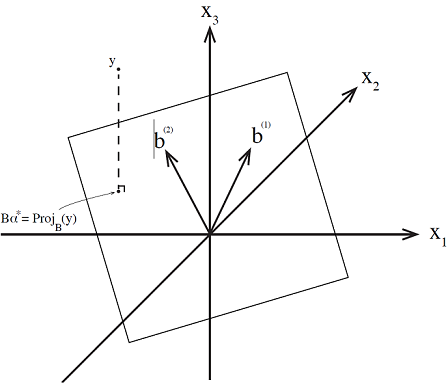
\includegraphics{proj2.png}

~

For \(n=6\), \(b_{0}\) through \(b_{5}\) are linearly combining to form
a plane Again, we want to find the point closest to \({\bm y}\). It will
be the point that is orthogonal and this point will be the
\(\text{Proj}_B(y)\).

~

The projection of \(x \in \mathbb{R}\) onto \(\Omega\) is the closest
point in \(\Omega\) to \(x\).

\begin{align*}
    P_\Omega(x) = \min_{z \in \Omega} ||z-x||
\end{align*}

Now suppose
\(\Omega = \text{Span}\left(b^{(0)} \ \ b^{(1)} \ \ \dots \ \ b^{(5)}\right)\),
and \(\displaystyle P_\Omega(x) = \min_{z \in \Omega} ||z-y|| \), where

\begin{align*}
     z &= \alpha_0 b^{(0)} + \alpha_1 b^{(1)} + ... + \alpha_5 b^{(5)} = B{\bm \alpha} = 
        \begin{pmatrix}
         b^{(0)} &  b^{(1)}& \dots & b^{(5)}
        \end{pmatrix}
        \begin{pmatrix}
        \alpha_0 & \alpha_1 & \dots & \alpha_5
        \end{pmatrix}^T
\end{align*}

and

\begin{align} \min_{z \in \Omega} ||z-y|| = \min_{z \in \Omega} ||\alpha_0 b^{(0)} + \alpha_1 b^{(1)} + ... + \alpha_5 b^{(5)}-y|| \end{align}

So we have \(\min\limits_{\alpha \in \mathbb{R}} ||B \alpha - y||^2\).
To tie projection and linear regression together, we can view linear
regression as a projection onto the span of the columns of the model
matrix.

~

Now tying both of them to quadratic optimization. When we have a linear
subspace and project onto it, it leads to a minimization of a quadratic
\(\min\limits_{\alpha \in \mathbb{R}^6} ||B{\bm \alpha}-{\bm y}||^2\),
(5) above. When \(\mathcal{F}\) is a linear function space then the
regression is a minimization of a quadratic
\(\min\limits_{\alpha \in \mathbb{R}^6 } ||{\bm y}-B{\bm \alpha}||^2\),
(4) above.

~

Both (4) and (5) are solved with the normal equations.

~

\begin{align*}
L(\alpha) &= \sum_{i=1}^N \left(   y_i - \alpha_0 + \alpha_1x_1^{(i)} + \alpha_2x_2^{(i)} + ... \alpha_nx_n^{(i)}  \right)^2 \\
&= \sum_{i=1}^N r_i^2 \\
&= {\bf r}\cdot{\bf r} \\
&=\left(y-B \alpha \right) \cdot \left(y-B \alpha\right) \\
&=\left(y-B \alpha\right)^T \left(y-B \alpha\right) \\
&= \left(y^T- (B \alpha)^T \right) \left(y-B \alpha\right) \\
&=y^Ty - (B\alpha)^Ty-y^TB\alpha + (B \alpha)^T B \alpha \\
&= y^Ty - 2(B^T y )^T  \alpha +\alpha^T B^T B \alpha \\
\\
\nabla L(\alpha) &= -\cfrac{1}{2} \left(B^T B \right)^{-1} \left(-2B^T y \right) \\
&= \left( B^T B \right)^{-1} B^T y
\end{align*}

We have shown that determining \(f(x)\) corresponds to a linear
regression, projection of a vector onto a linear space, and a quadratic
optimization.

\newpage

\begin{Shaded}
\begin{Highlighting}[]
\NormalTok{Fx<-}\ControlFlowTok{function}\NormalTok{(w,x)\{   }
    \CommentTok{#need this matrix for the normalizing Coefficients}
\NormalTok{    ncoef<-(}\DecValTok{1}\OperatorTok{/}\KeywordTok{sqrt}\NormalTok{( }\KeywordTok{diag}\NormalTok{(}\KeywordTok{Fapprox}\NormalTok{(}\DecValTok{1001}\NormalTok{,}\DataTypeTok{n=}\DecValTok{10000}\NormalTok{, bones}\OperatorTok{$}\NormalTok{age)) )) }
    \ControlFlowTok{if}\NormalTok{(w }\OperatorTok{==}\StringTok{ }\DecValTok{0}\NormalTok{ ) \{}\KeywordTok{return}\NormalTok{(   }\KeywordTok{rep}\NormalTok{(}\DecValTok{1}\NormalTok{,}\KeywordTok{length}\NormalTok{(x) ))  \} }\ControlFlowTok{else}\NormalTok{ \{}
    \KeywordTok{return}\NormalTok{( ncoef[w}\OperatorTok{+}\DecValTok{1}\NormalTok{]}\OperatorTok{*}\StringTok{ }\KeywordTok{cos}\NormalTok{( (}\DecValTok{2}\OperatorTok{*}\NormalTok{pi}\OperatorTok{*}\NormalTok{w}\OperatorTok{*}\NormalTok{(x}\OperatorTok{-}\FloatTok{9.4}\NormalTok{ ) ) }\OperatorTok{/}\NormalTok{(}\FloatTok{25.55}\OperatorTok{-}\FloatTok{9.4}\NormalTok{ )) )}
\NormalTok{        \} \}}
\NormalTok{dmat<-}\ControlFlowTok{function}\NormalTok{(m,}\DataTypeTok{n=}\DecValTok{10000}\NormalTok{,x)\{}

\NormalTok{MATT<-}\KeywordTok{matrix}\NormalTok{(}\DecValTok{0}\OperatorTok{:}\NormalTok{(m}\OperatorTok{-}\DecValTok{1}\NormalTok{),m,}\DecValTok{1}\NormalTok{)}

\NormalTok{dFx<-}\ControlFlowTok{function}\NormalTok{(v,x)\{ }\ControlFlowTok{if}\NormalTok{(v }\OperatorTok{!=}\StringTok{ }\DecValTok{0}\NormalTok{) \{}
    \KeywordTok{return}\NormalTok{( }\OperatorTok{-}\NormalTok{((}\DecValTok{4}\OperatorTok{*}\NormalTok{pi}\OperatorTok{^}\DecValTok{2}\OperatorTok{*}\NormalTok{v}\OperatorTok{^}\DecValTok{2}\NormalTok{)}\OperatorTok{/}\NormalTok{(}\FloatTok{16.15}\OperatorTok{^}\DecValTok{2}\NormalTok{))}\OperatorTok{*}\StringTok{ }\KeywordTok{cos}\NormalTok{( (}\DecValTok{2}\OperatorTok{*}\NormalTok{pi}\OperatorTok{*}\NormalTok{v}\OperatorTok{*}\NormalTok{(x}\OperatorTok{-}\FloatTok{9.4}\NormalTok{ ))}\OperatorTok{/}\FloatTok{16.15}\NormalTok{)}
\NormalTok{    )   \} }\ControlFlowTok{else}\NormalTok{  \{}\KeywordTok{return}\NormalTok{(}\KeywordTok{rep}\NormalTok{(}\DecValTok{1}\NormalTok{,}\KeywordTok{length}\NormalTok{(x) ))\} \}}

\NormalTok{a=}\KeywordTok{min}\NormalTok{(x);b=}\KeywordTok{max}\NormalTok{(x)}
\NormalTok{h=(b}\OperatorTok{-}\NormalTok{a)}\OperatorTok{/}\NormalTok{n;i=}\DecValTok{0}\OperatorTok{:}\NormalTok{(n}\OperatorTok{-}\DecValTok{1}\NormalTok{)}
\NormalTok{W<-}\KeywordTok{apply}\NormalTok{(MATT,}\DecValTok{1}\NormalTok{,}\ControlFlowTok{function}\NormalTok{(w) }\KeywordTok{dFx}\NormalTok{(w,a}\OperatorTok{+}\NormalTok{(i}\OperatorTok{+}\DecValTok{1}\NormalTok{)}\OperatorTok{*}\NormalTok{h) )  }
\NormalTok{\}}

\NormalTok{Bpp<-}\KeywordTok{dmat}\NormalTok{(}\DecValTok{1000}\OperatorTok{+}\DecValTok{1}\NormalTok{,}\DataTypeTok{n=}\DecValTok{10000}\NormalTok{, bones}\OperatorTok{$}\NormalTok{age)}
\NormalTok{z<-}\KeywordTok{seq}\NormalTok{(}\KeywordTok{min}\NormalTok{(bones}\OperatorTok{$}\NormalTok{age),}\KeywordTok{max}\NormalTok{(bones}\OperatorTok{$}\NormalTok{age),   }\DataTypeTok{length.out =} \DecValTok{10000}\NormalTok{ )}
\NormalTok{h<-z[}\DecValTok{2}\NormalTok{]}\OperatorTok{-}\NormalTok{z[}\DecValTok{1}\NormalTok{]}


\NormalTok{omega<-h}\OperatorTok{*}\NormalTok{(}\KeywordTok{t}\NormalTok{(Bpp) }\OperatorTok\StringTok{ }\NormalTok{Bpp )}

\NormalTok{B<-}\StringTok{ }\KeywordTok{model_matrix}\NormalTok{(bones}\OperatorTok{$}\NormalTok{age,}\DecValTok{1000}\NormalTok{)}
\NormalTok{n=}\DecValTok{1001}
\NormalTok{y<-}\KeywordTok{as.matrix}\NormalTok{( bones[,}\DecValTok{4}\NormalTok{] )}
\NormalTok{A<-}\KeywordTok{matrix}\NormalTok{(}\OtherTok{NA}\NormalTok{,(n ),}\DecValTok{3}\NormalTok{)}
\NormalTok{A[,}\DecValTok{1}\NormalTok{]<-}\KeywordTok{solve}\NormalTok{( }\KeywordTok{t}\NormalTok{(B)}\OperatorTok\NormalTok{B }\OperatorTok{+}\StringTok{ }\NormalTok{(.}\DecValTok{0001} \OperatorTok{*}\StringTok{ }\NormalTok{omega) ) }\OperatorTok\StringTok{ }\KeywordTok{t}\NormalTok{(B)}\OperatorTok\StringTok{ }\NormalTok{y}
\NormalTok{A[,}\DecValTok{2}\NormalTok{]<-}\KeywordTok{solve}\NormalTok{( }\KeywordTok{t}\NormalTok{(B)}\OperatorTok\NormalTok{B }\OperatorTok{+}\StringTok{ }\NormalTok{(}\DecValTok{1} \OperatorTok{*}\StringTok{ }\NormalTok{omega) ) }\OperatorTok\StringTok{ }\KeywordTok{t}\NormalTok{(B)}\OperatorTok\StringTok{ }\NormalTok{y}
\NormalTok{A[,}\DecValTok{3}\NormalTok{]<-}\KeywordTok{solve}\NormalTok{( }\KeywordTok{t}\NormalTok{(B)}\OperatorTok\NormalTok{B }\OperatorTok{+}\StringTok{ }\NormalTok{(}\DecValTok{100} \OperatorTok{*}\StringTok{ }\NormalTok{omega) ) }\OperatorTok\StringTok{ }\KeywordTok{t}\NormalTok{(B)}\OperatorTok\StringTok{ }\NormalTok{y}


\KeywordTok{par}\NormalTok{(}\DataTypeTok{mar=}\KeywordTok{c}\NormalTok{(}\FloatTok{4.1}\NormalTok{,}\FloatTok{4.1}\NormalTok{,}\DecValTok{1}\NormalTok{,}\DecValTok{1}\NormalTok{))}
\NormalTok{datt<-}\KeywordTok{data.frame}\NormalTok{(bones}\OperatorTok{$}\NormalTok{age, B}\OperatorTok\StringTok{ }\NormalTok{A[,}\DecValTok{1}\NormalTok{], B}\OperatorTok\StringTok{ }\NormalTok{A[,}\DecValTok{2}\NormalTok{], B}\OperatorTok\StringTok{ }\NormalTok{A[,}\DecValTok{3}\NormalTok{] )}
\NormalTok{datt<-datt[}\KeywordTok{with}\NormalTok{(datt, }\KeywordTok{order}\NormalTok{(bones}\OperatorTok{$}\NormalTok{age)), ]}

\KeywordTok{plot}\NormalTok{(bones[,}\DecValTok{2}\NormalTok{], bones[,}\DecValTok{4}\NormalTok{], }\DataTypeTok{xlab=}\StringTok{"age"}\NormalTok{, }\DataTypeTok{ylab=}\StringTok{"spnbmd"}\NormalTok{)}
\KeywordTok{lines}\NormalTok{( datt[,}\DecValTok{1}\NormalTok{],datt[,}\DecValTok{2}\NormalTok{],}\DataTypeTok{col=}\StringTok{"red"}\NormalTok{, }\DataTypeTok{lwd=}\DecValTok{2}\NormalTok{)}
\KeywordTok{lines}\NormalTok{( datt[,}\DecValTok{1}\NormalTok{],datt[,}\DecValTok{3}\NormalTok{],}\DataTypeTok{col=}\StringTok{"blue"}\NormalTok{, }\DataTypeTok{lwd=}\DecValTok{2}\NormalTok{)}
\KeywordTok{lines}\NormalTok{( datt[,}\DecValTok{1}\NormalTok{],datt[,}\DecValTok{4}\NormalTok{],}\DataTypeTok{col=}\StringTok{"green"}\NormalTok{, }\DataTypeTok{lwd=}\DecValTok{2}\NormalTok{)}
\end{Highlighting}
\end{Shaded}

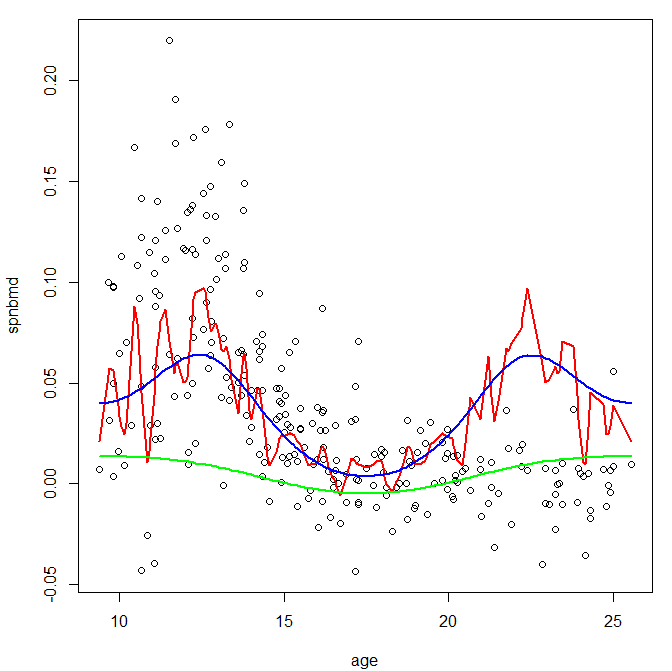
\includegraphics{penal.png}

As \(\rho\) increases the regression becomes more linear in order to
reduce the penalty term, the result is that the fitting term increases,
meaning that the fit becomes poorer.

\newpage

The neural net is a nonconvex optimization, we may go to a local
minimum. We want the hessian of the negative log likelihood to be
positive definite, or alternatively we want all the eigenvalues to be
positive. However, for neural nets the hessian of negative log
likelihood is not going to be positive definite because it is not a
convex function.

~

However we can modify the hessian such that it is positive definite and
similar to the hessian. We can rewrite the hessian as a decomposition,
and add a constant so the minimum eigenvalue becomes positive

\begin{align*}
     H&= Q \begin{pmatrix}
     \lambda_1  & &  \\
     & \lambda_2 &  \\
     & & \ddots &  \\
       &  &  &\lambda_n
     \end{pmatrix} Q^T \\
     \\
     H + \lambda I &= Q \begin{pmatrix}
     \lambda_1 + \lambda  & &  \\
     & \lambda_2 + \lambda&  \\
     & & \ddots &  \\
       &  &  &\lambda_n +  \lambda
     \end{pmatrix} Q^T \\
     \\
     &= Q \begin{pmatrix}
     \lambda_1  & &  \\
     & \lambda_2 &  \\
     & & \ddots &  \\
       &  &  &\lambda_n
     \end{pmatrix} Q^T+
     Q \begin{pmatrix}
     \lambda  & &  \\
     & \lambda &  \\
     & & \ddots &  \\
       &  &  &\lambda
     \end{pmatrix} Q^T.
 \end{align*}

We should raise \(\lambda\) if we are doing poorly, because raising the
lambdas enough will get all of our eigenvalues positive. When the
eigenvalues are all positive we are in a region of the function that is
locally convex and we will go down.

~

~

First, let's write down \(Hf(\eta)d\)

\begin{align}
     Hf(\eta)d &= \begin{pmatrix} \\[-.85em]
     \cfrac{ \ \partial^2 f(\eta) \ }{ \partial \eta_1^2} & \cfrac{ \ \partial^2 f(\eta) \ }{ \ \partial \eta_2 \partial \eta_1 \ } & ... & \cfrac{ \ \partial^2 f(\eta) \ }{ \ \partial \eta_n \partial \eta_1 \ } \\[1.25em]
     \cfrac{ \ \partial^2 f(\eta) \ }{ \ \partial \eta_2 \partial \eta_1 \ } & \cfrac{ \ \partial^2 f(\eta) \ }{ \ \partial \eta_2^2   \ } & ... & \cfrac{ \ \partial^2 f(\eta) \ }{ \ \partial \eta_n \partial \eta_2 \ } \\[1em]
     \vdots & \vdots & \ddots & \vdots \\[1em]
    \cfrac{ \ \partial^2 f(\eta) \ }{ \ \partial \eta_n \partial \eta_1 \ } & \cfrac{ \ \partial^2 f(\eta) \ }{ \ \partial \eta_n \partial \eta_2   \ } & ... & \cfrac{ \ \partial^2 f(\eta) \ }{ \ \partial \eta^2_n \ } \\[1.25em]
     \end{pmatrix} \begin{pmatrix} \\[-.85em] d_1     \\[1.25em] d_2  \\[1em] \vdots  \\[1em] d_n  \\[.85em]  \end{pmatrix} \\
     &= \begin{pmatrix} \\[-.85em]
     \cfrac{ \ \partial^2 f(\eta) \ }{ \partial \eta_1^2} \ d_1 + \cfrac{ \ \partial^2 f(\eta) \ }{ \ \partial \eta_2 \partial \eta_1 \ } \ d_2 + ... + \cfrac{ \ \partial^2 f(\eta) \ }{ \ \partial \eta_n \partial \eta_1 \ } \ d_n \\[1.25em]
     \cfrac{ \ \partial^2 f(\eta) \ }{ \ \partial \eta_2 \partial \eta_1 \ } \ d_1 + \cfrac{ \ \partial^2 f(\eta) \ }{ \ \partial \eta_2^2   \ } \ d_2  + ... + \cfrac{ \ \partial^2 f(\eta) \ }{ \ \partial \eta_n \partial \eta_2 \ } \ d_n \\[1em]
    \vdots \\[1em]
    \cfrac{ \ \partial^2 f(\eta) \ }{ \ \partial \eta_n \partial \eta_1 \ } \ d_1 + \cfrac{ \ \partial^2 f(\eta) \ }{ \ \partial \eta_n \partial \eta_2   \ } \ d_2 + ... + \cfrac{ \ \partial^2 f(\eta) \ }{ \ \partial \eta^2_n \ } \ d_n \\[1.25em]
     \end{pmatrix} \\
     &= \begin{pmatrix} 
    \\[-.85em]
   \nabla   \left( \cfrac{\partial }{\partial \eta_1 }  f(\eta) \right) \cdot {\bm d} \\[1.25em]
    \nabla   \left( \cfrac{\partial }{\partial \eta_2 }  f(\eta) \right) \cdot {\bm d} \\[1.25em]
    \vdots \\[1.25em]
    \nabla   \left( \cfrac{\partial }{\partial \eta_i }  f(\eta) \right) \cdot {\bm d} \\[1.25em]
    \vdots \\[1.25em]
    \nabla   \left( \cfrac{\partial }{\partial \eta_n }  f(\eta) \right) \cdot {\bm d} \\[1.25em]
    \end{pmatrix} 
 \end{align}

~

Now we can show that

\begin{align*}
     Hf(\eta)d &= \lim_{\epsilon \rightarrow 0} \cfrac{\nabla f(\eta + \epsilon d) - \nabla f(\eta)}{\epsilon} 
 \end{align*}

is equal to \(Hf(\eta)d\). Consider the \(i\)th coordinate of the vector
\(Hf(\eta)d\).

\begin{align}
     \Big[Hf(\eta)d\Big]_i &= 
     \lim_{\epsilon \rightarrow 0} \cfrac{ \ \cfrac{\partial }{\partial \eta_i }  f(\eta + \epsilon {\bm d}) -   \cfrac{\partial }{\partial \eta_i \ }   f(\eta)}{\epsilon}   
     \end{align}

First-order Taylor series expansion about the base point \(\eta\):

\begin{align*}
     \cfrac{\partial }{\partial \eta_i }  f(\eta + \epsilon {\bm d}) &\approx \cfrac{\partial }{\partial \eta_i }  f(\eta) + \nabla 
     \left( \cfrac{\partial }{\partial \eta_i }  f(\eta) \right) \cdot \epsilon {\bm d}. 
 \end{align*}

Plug back the expansion back into (9)

\begin{align*}
     \Big[Hf(\eta)d\Big]_i &= \lim_{\epsilon \rightarrow 0} \cfrac{ \ \cfrac{\partial }{\partial \eta_i }  f(\eta + \epsilon {\bm d}) -   \cfrac{\partial }{\partial \eta_i \ }   f(\eta)}{\epsilon}   \\
     \\
   & \approx \lim_{\epsilon \rightarrow 0} \cfrac{ \ \cancel{ \cfrac{ \partial }{\partial \eta_i }  f(\eta) } + \nabla 
     \left( \cfrac{\partial }{\partial \eta_i }  f(\eta) \right) \cdot \cancel{ \epsilon} {\bm d} - \cancel{ \cfrac{\partial }{\partial \eta_i \ }   f(\eta)} \ }{ \cancel{\epsilon }}   \\
     &= \nabla   \left( \cfrac{\partial }{\partial \eta_i }  f(\eta) \right) \cdot {\bm d}
\end{align*}

We see that for the \(i\)th coordinate is equal to the \(i\)th row in
(8) above. Other coordinates will follow by the same argument.


\end{document}
